% @author Arian Helberg

\chapter{Implementierung}
Zur Umsetzung der vorgestellten Konzepte wird im Folgenden auf Softwarepakete, Technologien, Datenspeicherung,
Benutzerinteraktion und Arbeitsablauf der erstellten Software eingegangen.
Darüber hinaus wird ein Überblick über Quellcode und einige Implementierungsentscheidungen gegeben.
Auf Implementierungsdetails zur Nutzung der vorgestellten Technologien wird nicht im Detail eingegangen.
Quellcode wird im Wesentlichen gezeigt und anhand von Zeilenangaben (z.B. \textbf{5}) erläutert.
Softwareumgebungsspezifische Implementierungsdetails werden unter Angabe von drei Punkten (\ldots) weggelassen.

\section{Projektstruktur}
Das Softwareprojekt ist nach der Gradle-Source-Code-Konvention organisiert.
Das gesamte Programm befindet sich im Ordner Generator, der obligatorische Gradle-Dateien und den
Source-Ordner enthält.
Sowohl die Quelldateien, also auch die Testdateien sind der Paketstruktur \textbf{de.haw} untergeordnet.
Die folgende Tabelle gibt einen Überblick über grundlegende Pakete und deren Funktion.

\begin{figure}[H]
    \centering
    \begin{tikzpicture}
        \draw[color=black!60!white]
        \FTdir(\FTroot,root,Generator){
            ++(0,-0.2em)
            \FTdir(root,src,src){
                ++(0,-0.2em)
                \FTdir(src,main,main){
                    ++(0,-0.2em)
                    \FTdir(main,java,java) {
                        ++(0,-0.2em)
                        \FTdir(java,de,de) {
                            ++(0,-0.2em)
                            \FTdir(de,haw,haw) {
                                ++(0,-0.5em)
                                \FTdir(haw,gui,gui) {
                                    ++(0,-0.5em)
                                    \FTdir(gui,shape,shape) {}
                                    ++(0,-0.5em)
                                    \FTdir(gui,structure,structure) {}
                                    ++(0,-0.5em)
                                    \FTdir(gui,template,template) {}
                                    ++(0,-0.5em)
                                    \FTdir(gui,turtle,turtle) {}
                                }
                                ++(0,-0.5em)
                                \FTdir(haw,lsystem,lsystem) {}
                                ++(0,-0.5em)
                                \FTdir(haw,pipeline,pipeline) {
                                    ++(0,-0.5em)
                                    \FTdir(pipeline,pipe,pipe) {}
                                }
                                ++(0,-0.5em)
                                \FTdir(haw,tool,tool) {}
                                ++(0,-0.5em)
                                \FTdir(haw,tree,tree) {}
                                ++(0,-0.5em)
                                \FTdir(haw,tree,utils) {}
                            }
                        }
                    }
                }

                \FTdir(src,test,test) {
                    \FTdir(test,java,java) {
                        \FTdir(java,de,de)
                    }
                }
            }
        };
    \end{tikzpicture}
    \caption{Softwareprojekt Dateistruktur}
\end{figure}

\begin{figure}[H]
    \centering
    \begin{tabular}{l|l}
        \textbf{Paket} &  \textbf{Funktion} \\ \hline
        \textit{gui} & Visualisierung des Programms \\ \hline
        \textit{lsystem} & L-System-Repräsentation \\ \hline
        \textit{pipeline} & Umsetzung des Pipeline-Design-Patterns \\ \hline
        \textit{tool} & Methodiken und Algorithmen \\ \hline
        \textit{tree} & Komponenten der Baumstruktur \\ \hline
        \textit{utils} & Hilfskomponenten
    \end{tabular}
    \caption{Softwarepakete mit zugehörigen Funktionen}
\end{figure}

\section{Technologien}
Zur Umsetzung des Softwarepojektes wird eine Java-Anwendung für die Java-Laufzeitumgebung entwickelt.
Sie liegt in der Distribution \textbf{Amazon Corretto} in der Version 11.0.3\_7 vor.
Grafische Oberflächen werden mit der JavaFX-Spezifikation von Oracle in der Version 11.0.2 umgesetzt.
Zur Automatisierung von Abhängigkeits- und Buildmanagement wird Gradle (Version 6.7) verwendet.
Eine Testumgebung, eine Vektorbibliothek, eine Tupelrepräsentation und eine Erweiterung zur mathematischen
Standartbibliothek werden über Abhängigkeiten vom Gradle-Framework im Build-Prozess geladen und zur Verfügung
gestellt.\\
Um den test-driven Implementierungsansatz umzusetzen wird JUnit 5 Jupiter als Testumgebung genutzt.
Sie setzt sich aus einem Programmierschema und einem Erweiterungsmodell zusammen.
Das Jupiter-Projekt liefert zudem die Laufzeitumgebung für Softwaretests.
Googles Guava liefert eine Bibliothek mit mathematischen Funktionen.
Sie wird benötigt, um eine praktikable Lösung zu Mengenmanipulation nutzen zu können (Bsp. Erstellen
von Kombinationspaaren einer Menge).
Ausschließlich JavaFX wird außerhalb des Projektes installiert und als Modul im Start-Skript des Programmes
hinzugefügt.
\\~\\
Weitere Systeme zur Erstellung des Softwareprojektes sind:
\begin{itemize}
    \item Versionierung via Git,
    \item Dot zur Visualisierung von Graphen und
    \item PlantUML zur Generierung von UML-Diagrammen
\end{itemize}

\newpage

\section{Konzeptumsetzung}

Das Skript \texttt{Generator.bat}, das zum Starten der Anwendung innerhalb eines Windows-Betriebssystems genutzt werden kann,
fügt dem Programm alle externen Module hinzu, die während der Laufzeit genutzt werden, und führt die angegebene jar-Datei aus:
\begin{figure}[H]
    \centering
    \begin{csource}
    java --module-path .\javafx-sdk-11.0.2\lib --add-modules javafx.controls,javafx.fxml,javafx.graphics -jar Generator-1.0.jar
    pause
    \end{csource}
    \caption{Startskript Generator.bat}
\end{figure}

Beim Start der Anwendung findet der Benutzer die grafische Oberfläche vor.
\begin{figure}[H]
    \centering
    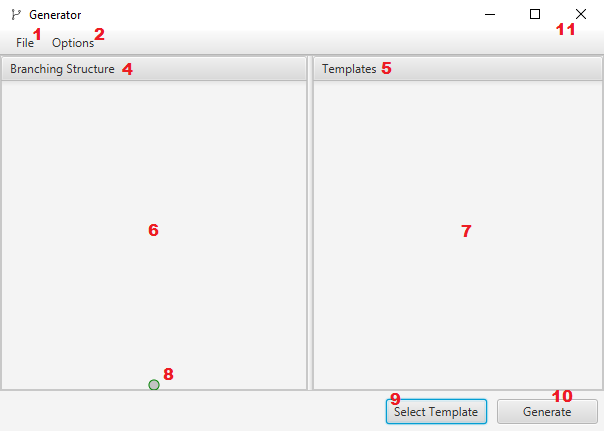
\includegraphics[width=14cm]{../images/UI_numbers1.png}
    \caption{Programm nach Ausführung des Start-Skripts}
\end{figure}
Der Menüeintrag \textbf{1} bietet Funktionen zum Öffnen des Dateipfades und zum Laden der angelegten Templates-Datei.
\textbf{2} dient zur Konfiguration der Umgebungsparameter für die Anzahl Iterationen der Ausführung
und die Anzahl an Ähnlichkeitsstrukturen, die aus dem resultierenden L-System abgeleitet werden können.
Die Gewichtungsparameter der vorgestellten Algorithmen können ebenfalls hier eingestellt werden.
Die Strukturen \textbf{4} und \textbf{5} gliedern das Programm in die Ansicht der Verzweiungsstruktur (\textbf{6}), die vom Benutzer
angelegt wird, die Übersicht zur Auswahl eines Templates (\textbf{7}) und eine Sicht zur Setzung von Transformationsparametern (\textbf{7}).
Der Kreis \textbf{8} stellt einen Anker dar, an welchen eine Template-Instanz angehängt werden kann.
Sowohl über einen Doppelklick, also auch über einen Button (\textbf{9}) kann ein Template aus der Tempalte-Liste (\textbf{7})
ausgewählt werden.
Ist die Verzweigungsstruktur vom Benutzer fertiggestellt, kann die Synthese zur Erstellung der Ähnlichkeitsabbildungen
mit \textbf{10} erfolgen.
Wird der Generieren-Button ohne eine Basisstruktur gedrückt, lässt sich das Beispiel aus
dieser Arbeit erzeugen (ohne visualisierung der Basisstruktur).
\textbf{11} schließt die Anwendung.

\subsection*{Templates}
Eine Datei \textit{template.txt} wird im selben Verzeichnis wie die ausführbare jar-Datei hinerlegt.
Die enthält je eine Template-Zeichenkette pro Zeile, die vom Programm eingelesen und als Template
zur Verfügung gestellt wird.
\begin{figure}[H]
    \centering
    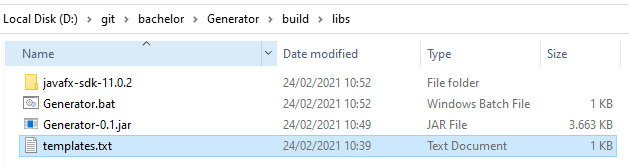
\includegraphics[width=12cm]{../images/templates_file.png}
    \caption{Tempaltes-Datei zum Einlesen der Template-Strukturen}
\end{figure}

\newpage

\subsection*{Visualisierung}
Die grafische Oberfläche liegt als MVC-Pattern in Form des Application State (Model), der XML-basierten FXML-Datei (View)
und dem JavaFX-Controller vor.
Der Arbeitsablauf zur Erstellung der Verzweigungsstruktur kann Schritt für Schritt umgesetzt werden, nachdem die Templates
geladen wurden.
Dies wird an folgendem Beispiel deutlich gemacht.
Die Parameter \textbf{Number of iterations}, \textbf{Number of generations}, \textbf{Rule application ratio} und
\textbf{Merge application ratio} werden auf die Werte \textbf{5}, \textbf{5}, \textbf{0.5} und \textbf{0.5} gesetzt
(Standardeinstellung).
\begin{figure}[H]
    \centering
    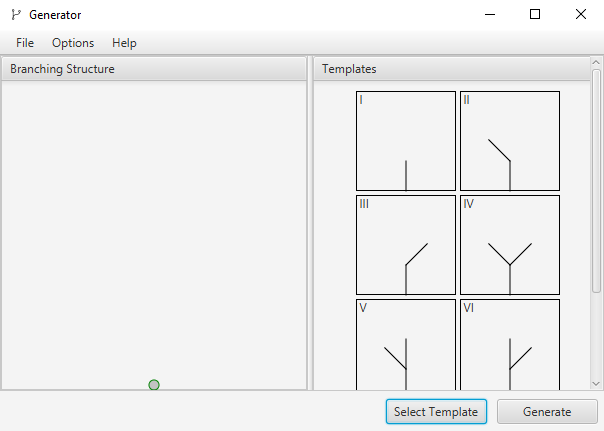
\includegraphics[width=6cm]{../images/UI_templates.png}
    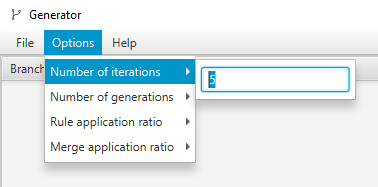
\includegraphics[width=6cm]{../images/UI_parameters.png}
    \caption{Erster Anker ist vorselektiert \& gesetzte Parameter}
\end{figure}

\begin{figure}[H]
    \centering
    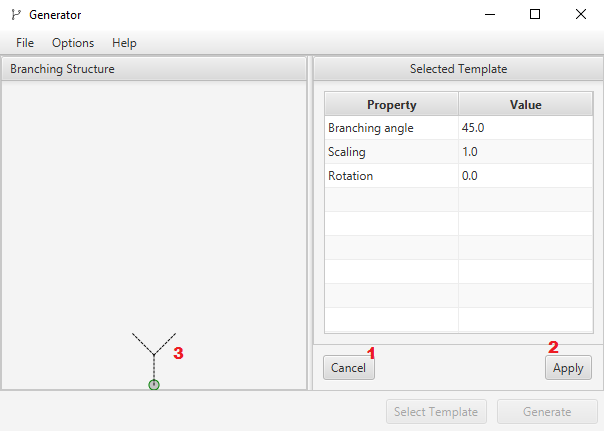
\includegraphics[width=12cm]{../images/UI_template.png}
    \caption{Auswahl des ersten Templates}
\end{figure}

Nachdem ein Template ausgewählt wurde, können die Transformationsparameter gesetzt (Doppelklick) werden und die Auswahl
rückgängig gemacht (\textbf{1}) oder bestätigt (\textbf{2}) werden.
\textbf{3} zeigt einen Entwurf der Tempalte-Instanz, die mit den aktuellen Transformationsparametern angepasst wurde.
Mit der Bestätigung wird die Template-Instanz endgültig der Basisstruktur hinzugefügt und der Benutzer gelangt wieder
in die Übersich der zur Verfügung stehenden Templates.
\begin{figure}[H]
    \centering
    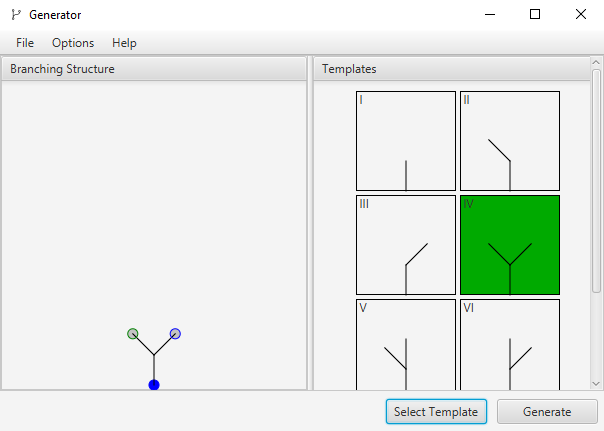
\includegraphics[width=12cm]{../images/UI_applied.png}
    \caption{Der Verzweigungsstruktur hinzugefügte Template-Instanz}
\end{figure}

Dieser Vorgang wiederholt sich, bis der Benutzer die Struktur fertiggestellt hat.
\begin{figure}[H]
    \centering
    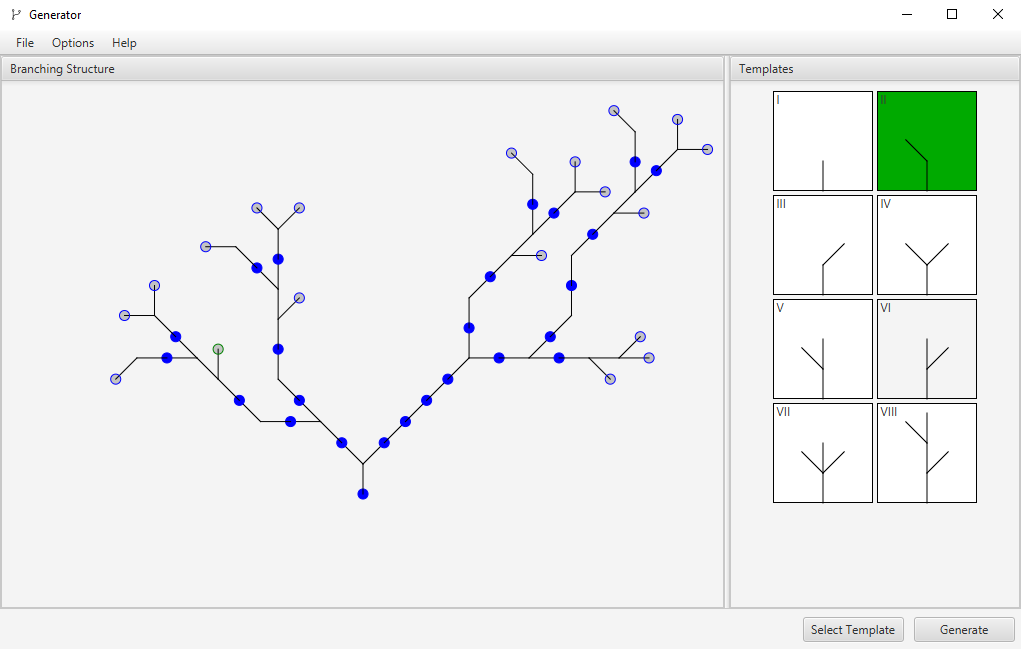
\includegraphics[width=13cm]{../images/UI_finished.png}
    \caption{Vom Benutzer fertiggestellte Verzweigungsstruktur}
\end{figure}

Über den \textbf{Generate}-Button kann nun die Synthese gestartet werden.
Es ergeben sich 5 (\textbf{Number of generations}) Ähnlichkeitsstrukturen
(siehe ~\ref{resulting_structures})

\subsection*{Baumtopologie}
Um eine interne Baumtopologie aufzubauen wird die Klasse \texttt{TreeNode} verwendet, um eine iterierbare Baumstruktur
aufzubauen (siehe~\ref{treestructure}).
\texttt{TreeNode} implementiert die \texttt{Iterable}-Schnittstelle, was ein Überladen der \texttt{iterator}-Funktion möglich
macht.
Sie stellt einen Iterator des Baumes zur Verfügung.
Dieser Iterator (\texttt{TreeNodeIterator}) implementiert die \texttt{Iterator}-Schnittstelle und definiert so die Funktionen
\texttt{hasNext} und \texttt{next}.
Die Funktion \texttt{next} zeigt, wie eine Iteration des Baumes als Breitensuche implementiert ist.
Diese wird beim Inferieren eines L-Systems aus der Baumstruktur benötigt (siehe~\ref{iterator}).

\newpage

Das folgende Beispiel zeigt eine erstellte Baumstruktur (links) und deren erstellte Baumtopologie (rechts).
\begin{figure}[H]
    \centering
    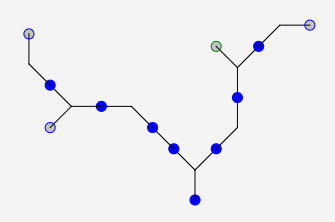
\includegraphics[width=8cm]{../images/graph_tree.png}
    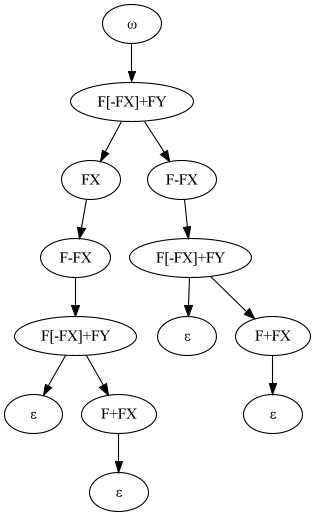
\includegraphics[width=5cm]{../images/tree_graph.png}
    \caption{Verzweigungsstruktur \& zugehörige Baumstruktur}
\end{figure}

\subsection*{Prozesspipeline}
Das angewendete Pipeline-Design-Pattern zur Umsetzung der Inferrierung, Komprimierung und Generalisierung von L-Systemem,
sowie der Verteilung von Transformationsparametern bei deren Ausführung, setzt sich aus der \texttt{Pipeline}-Klasse und
dem \texttt{Pipe}-Interface zusammen (siehe~\ref{pipeline1} und~\ref{pipeline2}).\\~\\
Die eigentliche Umsetzung der Prozesspipeline zur Synthese der Verzweigungsstrukturen wird wie folgt implementiert.
Hierbei implementieren die Klassen \texttt{InfererPipe}, \texttt{CompressorPipe}, \texttt{GeneralizerPipe} und
\texttt{EstimatorPipe} das \texttt{Pipe}-Interface und geben die Reihenfolge des Prozesses an.
Das \texttt{ctx}-Objekt wird als Kontextobjekt in die Pipeline gegeben und bei jedem Prozessschritt angepasst (siehe~\ref{ctx}).

\subsection*{L-System Manipulation}
Die Inferrierung des L-Systems findet in der Klasse \texttt{Inferer} statt, die in der \texttt{InfererPipe}-Klasse erstellt wird.
Sie nimmt die Baumstruktur entgegegen und stellt eine Funktion \texttt{infer} zum Inferieren des L-Systems zur Verfügung (siehe~\ref{inferer}).\\
Das erstellte L-System (\textbf{8}) wird während des Inferierens aktualisiert und am Schluss als Ergebnis zurückgegeben.
Dann werden die initialen Symbole $F$ und $S$ hinzugefügt und das Axiom auf $S$ gesetzt (\textbf{10-12}).
Die initiale Produktionsregel $\alpha: S \rightarrow A$ wird erstellt und der Produktionsregelmenge beigefügt (\textbf{14-15}).
Es wird der erste zu untersuchende Knoten des Baumen über seinen Iterator zurückgegeben und als $\beta$ gesetzt (\textbf{17}).
Am Ende der Initialisierung fügt die Methode \texttt{addModuleNotPresentInAlphabet} dem Alphabet ein neues Symbol (\texttt{gamma}) hinzu,
das dort nicht vorhanden ist (\textbf{19}).
Dies geschieht nach lexikografischer Reihenfolge.

Nach der Erstellung des \texttt{Inferer}-Objektes kann in der zugehörigen Pipe \texttt{InfererPipe} das L-System inferriert
werden (siehe~\ref{infererpipe}).\\~\\
Für die Implementierung des Inferrierungsalgorithmus siehe~\ref{infer}.\\
Die \texttt{infer}-Methode extrahiert die Zeichenkette (Wort) des im aktuellen Baumknoten gespeicherten Template-Instanz
(\textbf{9}) und speichert sie zur Bearbeitung in \texttt{delta}.
Delta wird nach Verzweigungsvariablen durchsucht (\textbf{11-14}) und diese dann durch ein neues Symbol,
das dem Alphabet hinzugefügt wird (\textbf{18}), ersetzt (\textbf{20}).
Eine neue Produktionsregel, die \texttt{gamma} auf das veränderte Wort abbildet, wird dem L-System beigefügt (\textbf{24}).
\textbf{31-35} sucht nach Symbolen im Alphabet, die noch kein Ziel einer Produktionsregel sind und hält diese in der
Variablen \texttt{gamma}.
Wird kein solches Symbol gefunden, terminiert die \texttt{infer}-Methode und damit der Algorithmus (\textbf{44}).
Der aktuelle Knoten wird durch den Iterator der Baumstruktur mit dem nächsten Knoten nach Breitensuche ersetzt (\textbf{46}).
Zum Schluss wird das inferrierte L-System zurückgegeben (\textbf{48}).\\

Die übrigen Prozessschritte sind ähnlich aufgebaut.
Auch die Klassen \texttt{Compressor}, \texttt{Generalizer} und \texttt{Estimator} implementieren eine Funktion zum Ausführer
der jeweiligen Algorithmen, während die Initialisierung im Konstruktor ausgeführt wird.
Dabei wird die Implementierung der Algorithmen eng an der Konzeptionierung gehalten (siehe Kapitel ~\ref{algo}).
Alle weiteren Klassen der Basisalgorithmen werden in~\ref{komp} bis~\ref{durchschnittparameter} gezeigt.
Der Algorithmus \texttt{editDistanceOptimized} aus~\ref{editdistance} ist aus Praktikabilitätsgründen aus~\cite{editdistance}
entnommen.